\chapter{Adapting Behavior} \label{chap:systemOverview}

The implication of a physical agent, like Nao, in a human-child interaction context provide several benefits (see chapter \ref{chap:litReview}). It is important to be able to use all resources such as arms, head and other in an adaptive and flexible way without modifying the essence of the main activity, the writing. Therefore, the final goal of an adaptive behaviour is to smooth the interaction with the purpose to make children show more positive attitude towards the activity presented \cite{lim2014mei}\cite{tielman2014adaptive}. In this sense, an adaptive emotion expression system was developed based on internal valance and arousal values influenced by the current state of the interaction partner.

In addition, most of the visual information extracted from the user during the interaction will be recorded and used to assess the level of engagement. Therefore, we hypothesize that some of the features captured such as quantity of movement, proximity or gaze direction can be identifiers of the engagement level in this specific interaction context. The results related to this second part are shown in chapter \ref{chap:feasibility}.

\section{The valence and Arousal model}
	
The valence-arousal model has been widely spread as a simple standard for emotion detection and modelling in the literature \cite{russell1980circumplex}. Valence refers to how positive or negative an event is, and arousal reflects whether an event is exciting or calming, agitating or soothing. In this case, this technique is applied to enrich the variety of behaviours expressions based on online factors coming from the user interacting.

The main principle of the model is the need to be feed with external information which is encoded along two dimensions, \textit{valence} and \textit{arousal}. These dimensions are represented on a scale from -1 to 1 and are used to physically modify the current behaviour of the robot. For instance, when the child smiles to the robot, the current emotion indicator moves towards \textit{happiness} encoded in the map shown in figure \ref{fig:vaMap}.

\begin{figure}[h!]
        \centering
        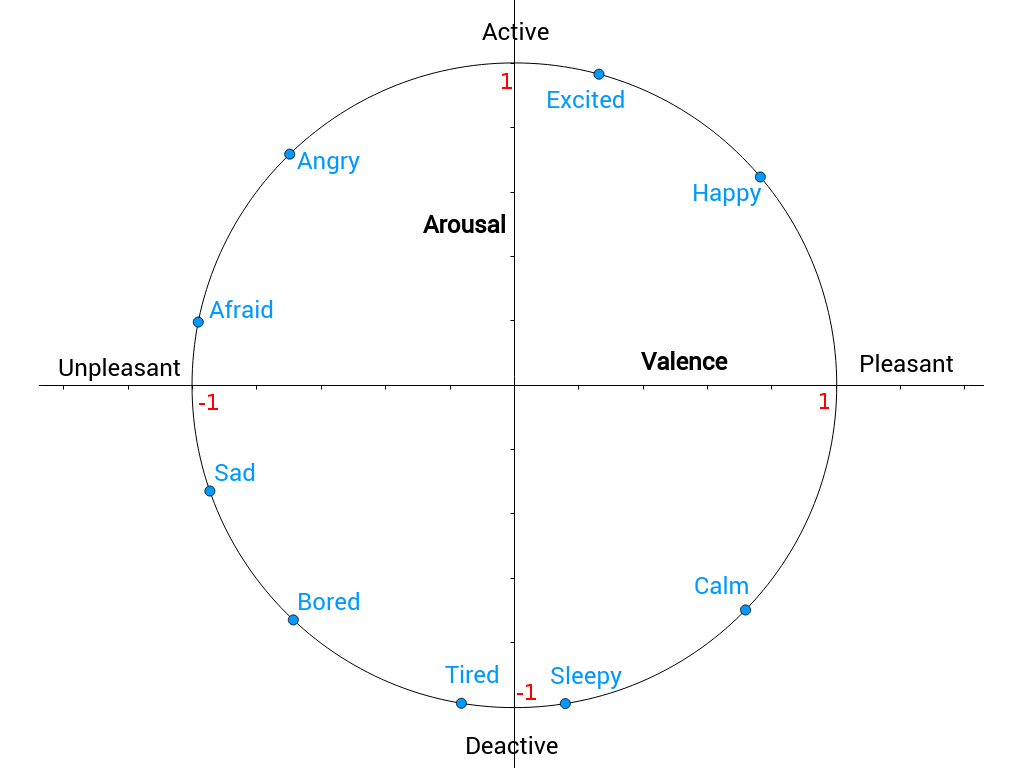
\includegraphics[width=0.6\textwidth]{figures/vaMap.png}
        \caption{Valence-Arousal map \cite{bradley1999affective}}
        \label{fig:vaMap}
\end{figure} 
  
\section{System Overview} \label{SystemOverview}

In order to capture the appropriate cues from the children with the purpose of generating an emotion content in a 2D map, we relied on \textit{dlib} library. This resource, in combination with the tools offered by OpenCV, provide the sufficient robustness to reliably acquire user faces. Once the acquisition tools and the behaviour model are established, it is necessary to define the possible visual relevant cues: 

\begin{itemize}
  \item Proximity to the scene.
  \item Quantity of movement (QoM).
  \item Gaze direction.
  \item Saliency.
  \item Beaming.
\end{itemize}

And the generation of a set of behaviours on the humanoid robot Nao based on the following actuators:

\begin{itemize} \label{listResources}
  \item Head pitch
  \item Left and right shoulder roll and pitch.
  \item Left and right elbow roll.
  \item LED eye color.
  \item Pitch and volume voice.
\end{itemize}

The main challenge is to combine the behaviour adaptation together with other independent activities since in both cases resources such as arms or head are shared between them. It is a must not to collide with the current activity but still adapt the behaviour of the robot on real time. At this point the implementation of the system plays an important role. It has been divided in three ROS nodes; the \textit{vision} manager, the \textit{emotion manager}, and the \textit{action} manager. The framework is designed in such a way that its execution is independent from the original CoWriter, acting as a modifier and activity independent (see figure \ref{fig:system}).

\bigskip

\begin{figure}[h!]
        \centering
        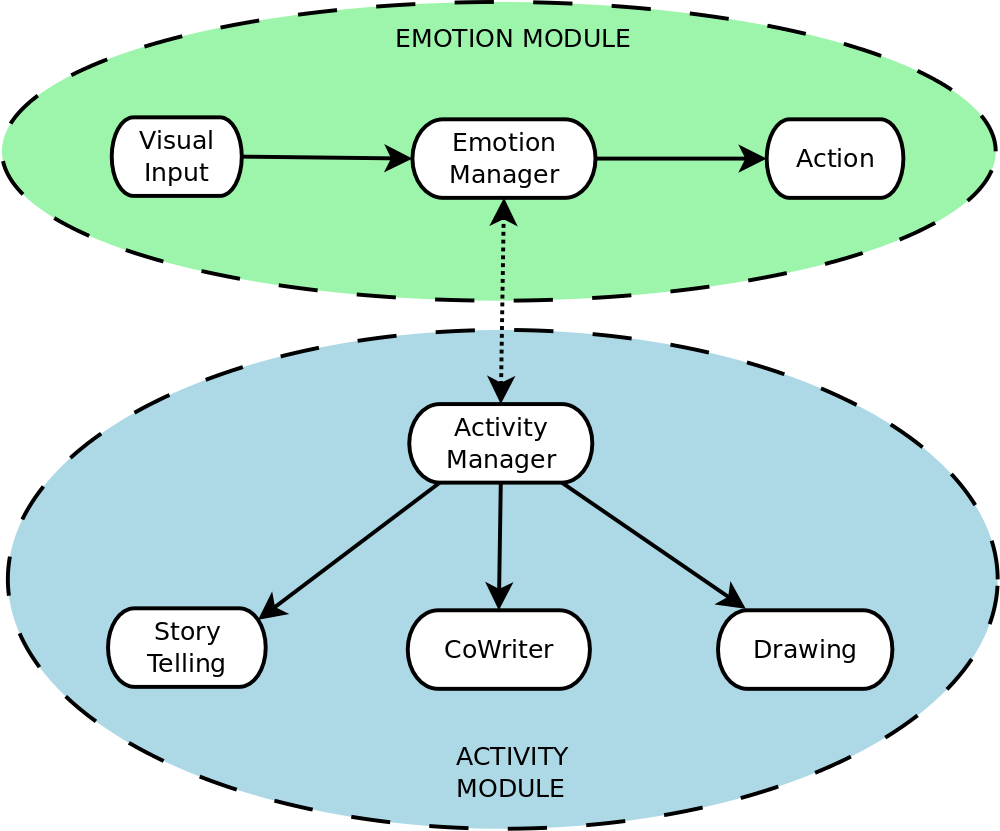
\includegraphics[width=0.5\textwidth]{figures/system.png}
        \caption{Independent emotion (green) and activity (blue) frameworks}
        \label{fig:system}
\end{figure}

\bigskip

The \textit{vision} node is written in C++ and contains all computation related with the image acquisition and processing using both OpenCV and \textit{dlib}. It publishes to the \textit{emotion manager} node which integrates all the information received and generates a resultant vector (valence-arousal) towards the correspondent emotion. Finally, the \textit{action} node performs the necessary movements to embody the emotion at the specific time. A deeper overview of the system is shown in figure below.

\begin{figure}[h!]
  \begin{adjustbox}{addcode={\begin{minipage}{\width}}{\caption{%
      Structure of the ROS nodes used to implement the system. Ovals represent nodes, arrows represent messages, and rectangles message topics.
      }\end{minipage}},rotate=90,center}
      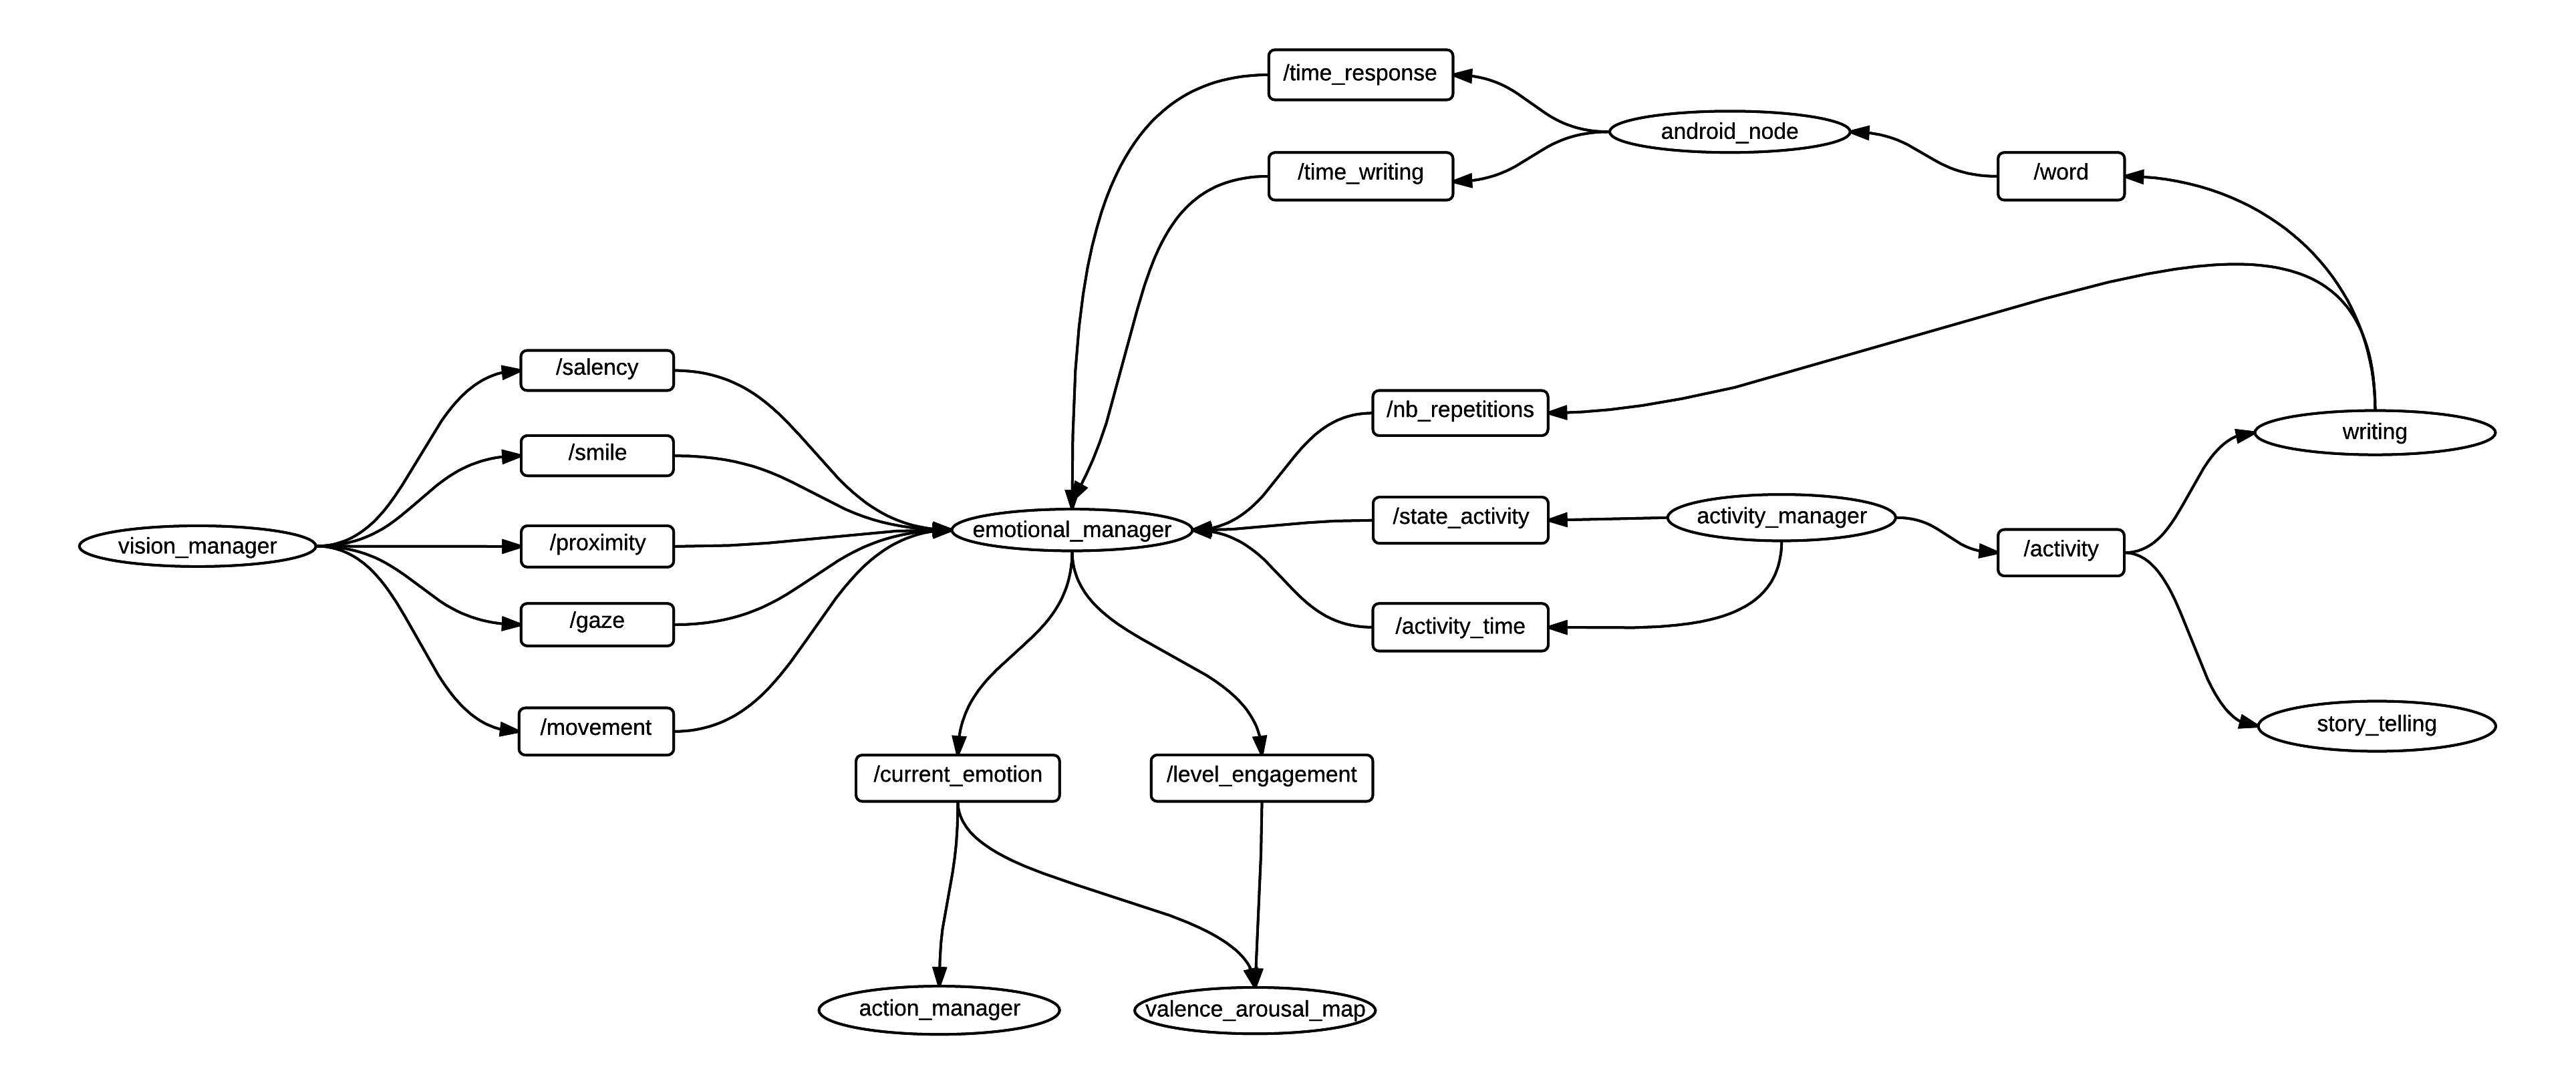
\includegraphics[scale=.57]{figures/chart.png}%     
  \end{adjustbox}
\end{figure}

\section{Vision node}
The \textit{vision} node is responsible for everything related with the features acquisition and image processing. Proximity to the robot, quantity of movement, gaze direction, smiles and saliency are the cues extracted from the scene. They will be explained in detail in the following sections. Each of them generates a 2D valence-arousal vector towards a specific behaviour.

As we previously mention, \textit{dlib} allow us to perform face pose estimation very quickly adding face landmarks to the image captured (see figure \ref{fig:dlib}).

\begin{figure}[!htb]
        \centering
        \begin{tikzpicture}[>=latex]
        	\node[inner sep=0pt] (xtion) at (0,0) {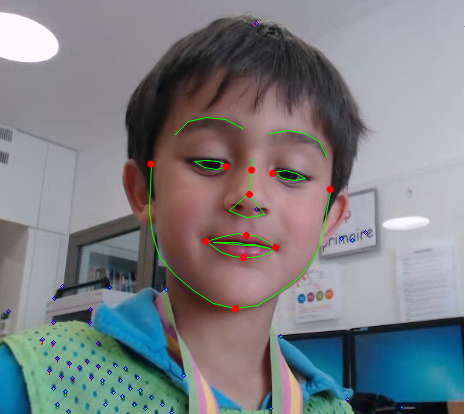
\includegraphics[width=.8\textwidth]{figures/faceMark.png}};
        	
    		\node[red, text width=1.5cm] at (-2.2,1.1) {$side_L$};
    		\node[red, text width=1.5cm] at (3.2,0.6) {$side_R$};
    		\node[red, text width=1.5cm] at (1,1.2) {$up$};
    		\node[red, text width=1.5cm] at (0,-2.7) {$chin$};
    		\node[red, text width=1.5cm] at (1.7,1.1) {$eye_R$};
    		\node[red, text width=1.5cm] at (0,1.3) {$eye_L$};
		    \node[red, text width=1.5cm] at (0.5,-0.5) {$mouth_U$};
		    \node[red, text width=1.5cm] at (0.5,-1.6) {$mouth_D$};
		    \node[red, text width=1.5cm] at (2,-1.2) {$mouth_R$};
		    \node[red, text width=1.5cm] at (-1.2,-1) {$mouth_L$};
		    \node[red, text width=1.5cm] at (1,0.5) {$nose$};
        			
       	\end{tikzpicture}
        \caption{\textit{dlib} face landmarkers in a subject experiment}
        \label{fig:dlib}
\end{figure}


\subsection{Proximity to the scene}
Back posture has been proved to be a reliable indicator of user's engagement \cite{d2007posture} \cite{castellano2009detecting}. We believe that this is directly correlated with the proximity towards the region of interaction composed, in this case, by Nao and a tablet. This can be estimated using the size of the face and it is interpreted as a positive reaction and thus, the behaviour shown is positive too (see figure \ref{fig:vaMap}). Moreover, this measurement will be recorded during the whole interaction and analysed as a possible indicator of activity engagement.

In order to be estimated, it is necessary to compute the middle point between the eyes because it decreases the variability due to the movement like in equation \ref{eq:proximity}.

\begin{equation} \label{eq:proximity}
up(x,y) = \left (\frac{eye_{L}(x)-eye_{R}(x)}{2}, \frac{eye_{L}(y)-eye_{R}(y)}{2}\right )
\end{equation}

Then, the distance in the vertical line of the face can be computed using $ up(x,y) $ and $ chin(x,y) $ as in equation \ref{eq:proximity2}:

\begin{equation} \label{eq:proximity2}
d(up,chin) = \sqrt{({(up(x)-chin(x))}^2 + {(up(y)-chin(y))}^2)}
\end{equation}

The result will induce a positive behaviour in case the child show proximity to the robot.

\subsection{Quantity of movement}
The quantity of movement, like the proximity, is captured and kept during the interaction. However, as happens with the proximity, it is also useful to model behaviour responses with Nao. In order, to catch the movement from the scene, several methods were tested. We selected a method based on optical-flow since it is less sensitive to image noise than point-wise methods.

The algorithm finds the most prominent corners in the image computing the corner Minimum Eigenvalue as described in \cite{shi1994good}, which stores the minimal eigenvalue of a block size neighbourhood \textit{S(p)}, that is, $ \min(\lambda_1, \lambda_2) $ in terms of the following equation:

\begin{equation}
M =  \begin{bmatrix} 
		\sum _{S(p)}(dI/dx)^2 &  \sum _{S(p)}(dI/dx dI/dy)^2  \\ 
		\sum _{S(p)}(dI/dx dI/dy)^2 &  \sum _{S(p)}(dI/dy)^2 
	 \end{bmatrix}
\end{equation} 

where the derivatives are computed using the \textit{Sobel} operator. After that, it finds the minimum eigenvalue of \textit{M} and stores them.

Once the relevant points are detected, the second step is to calculate the flow from these points. The technique used is based on Lucas-Kanade method with pyramids implemented in OpenCV \cite{bouguet2001pyramidal} which assumes that the flow is essentially constant in a local neighbourhood of the pixel under consideration and solves the basic optical flow equations for all the pixels in that neighbourhood by the least squares criterion. Being the equations formulated as in \ref{lucasKanade}.

\begin{equation} \label{lucasKanade}
A =  \left( \begin{array}{cc}
	I_x(q_1) & I_x(q_1) \\
	I_x(q_1) & I_x(q_1) \\
	\colon & \colon  \\
	I_x(q_n) & I_x(q_n)
	\end{array} \right),
\qquad  
v =  \left( \begin{array}{cc}
		V_x  \\
		V_y \\
	\end{array} \right),
\qquad	 	 
b =  \left( \begin{array}{c}
	 		-I_t(q_1)\\
	 		-I_t(q_2)\\
	 		\colon \\
	 		-I_t(q_n)\\
	 \end{array} \right)
\end{equation}

This system has more equations than unknowns and thus it is usually over-determined. So, needs to be reformulated as shown in \ref{lucasKanade1}. 

\begin{equation} \label{lucasKanade1}
A^TAv = A^Tb
\qquad
\Rightarrow
\qquad
v=(A^TA)^{-1}A^Tb
\end{equation}

In the final analysis, the result can be seen in figure \ref{fig:optical}. In this case the high quantity of movement is interpreted as a negative input inducing an angry behaviour.

\begin{figure}[h!]
        \centering
        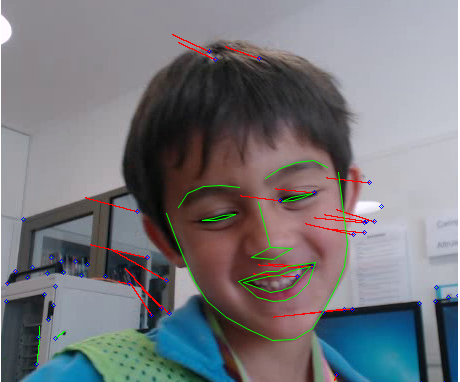
\includegraphics[width=0.5\textwidth]{figures/optical.png}
        \caption{Optical flow output in a real interaction context}
        \label{fig:optical}
\end{figure}

\subsection{Gaze direction}
The gaze direction was computed using a simple but effective method through the landmark positions provided by the face pose estimation. As it happens with the quantity of movement, as well as with the proximity, the data acquired is interpreted for both, behaviour adaptation and engagement assessment.

First, we compute the length of the segments between the right and the left face sides ($ side_R $ and $ side_L $, respectively) with respect to the nose, $ d(nose,side_R) $ and $ d(nose,side_L) $, as well as the distance between both sides, $ d(side_R,side_L) $. So, it results in equation \ref{eq:estwest},

\begin{equation} \label{eq:estwest}
horizontal = \frac{d(nose,side_R)-d(nose,side_L)}{d(side_R,side_L)}
\end{equation}

where the result is normalized in the range $ [-1,1] $. A value greater than a threshold of 0.3 indicates \textit{left} as gaze direction, whereas lower than -0.3 indicates \textit{right} direction.

Second, we perform a similar operation to detect when a user is looking up or down. It is necessary to calculate the projection of the nose position in the \textit{horizontal} segment that goes from $ side_R $ to $side_L$ like in equations \ref{eq:projection} and \ref{eq:projection1}.

\begin{equation}\label{eq:projection}
d_{proj} = d(nose,side_R) \cdot \left(\frac{horizontal}{d(nose,side_R)} + d(nose,side_L)\right )
\end{equation}

\begin{equation} \label{eq:projection1}
proj(x,y) = \frac{P_{side_R}(x,y)+(P_{side_L}(x,y)-P_{side_R}(x,y))\cdot d_{proj}}{horizontal}
\end{equation}

Then, we can compare if the height of $ proj(x,y) $ is greater or lower than the nose position with a certain tolerance. If it is the case, the user is looking up or down respectively. Finally, if none of the directions is satisfied, we assume that the user is looking straight at the robot inducing a positive behaviour.


\subsection{Saliency}

The \textit{saliency} is a concept that is related with the changes on the current state of the scene. Events such as a new person detected in the scene as well as quick movements after a period of tranquility or vice-versa, are considered as a novelty. It can be used to modify the current status of the robot towards a \textit{surprise} behaviour.

The algorithm implemented for this detection consist on the Exponential Moving Average (EMA), defined in equation \ref{eq:EMA},

\begin{equation} \label{eq:EMA}
 t > 1,\ \    S_{t} = \alpha \cdot Y_{t} + (1-\alpha) \cdot S_{t-1}
\end{equation}

where,

\begin{itemize}
\item The coefficient $ \alpha $ represents the degree of weighting decrease, a constant smoothing factor between 0 and 1. A higher $ \alpha $ discounts older observations faster.
\item $ Y_t $ is the value at a time period \textit{t}.
\item $ S_t $ is the value of the EMA at any time period \textit{t}.
\end{itemize}

Once the EMA $S_t$ value is computed, the distance with respect to the previous EMA, $S_{t-1}$ needs to be computed of course, for each kind of event (gaze, proximity...), as shown in equation \ref{eq:EMA2}.

\begin{equation} \label{eq:EMA2}
d = \frac{(S_t - S_{t-1})^2}{\epsilon + (S_t + S_{t-1})^2 }
\end{equation}

When a high quantity of movement is captured after a period without movement, a new face is detected, or the proximity changes in great manner, it produces a behaviour response in the field of surprise.

\subsection{Child smiles}
In order to capture the smile of the children, it has been necessary to calculate the intersection between the segment composed by the two mouth corners, $ mouth_L $ and $ mouth_R $, and the vertical ones, $mouth_U$ and $mouth_D$. Whenever there is no intersection is due to a smile: The segment composed by $mouth_U$ and $mouth_D$ is above the $mouth_U$ point. However, the detections are restricted to the robot eye contact situations only, helping to induce a happy behaviour.


\section{Emotion manager node}
This node is responsible for the vectorization of the incoming information from the \textit{vision} node and eventually, the computation of the correspondent valence and arousal values. Furthermore, besides the features extracted from the \textit{vision} module, there are additional ones such as; the time spend in the activity or the number of repetitions that have an influence in the resulting vectorization of the current state (see figure \ref{fig:vectMap}). The summary of the cues used, the direction of the correspondent vectors (valence, arousal) assuming an initial point $ (0,0) $, the weight of them in the final computation, as well as the cues that are used for the engagement assessment are shown in table \ref{tab:cues}.

\begin{table}[h!]
\centering
\begin{tabular}{l|l|l|l|l}
 \textbf{Features}   & \textbf{Valence}  & \textbf{Arousal}  & \textbf{Weight} & \textbf{Engagement}\\ \hline	
 \textit{QoM}  	  		  	 &   -1 	      	 &    1 	& 14\% &   +  \\ \hline
 \textit{Proximity}    	  	 &   1  	      	 &    1		& 7\%  &   +  \\ \hline
 \textit{Saliency}	  	  	 &   0 	      		 &    1 	& 7\%  &   +  \\ \hline
 \textit{Gaze: robot contact} 	 &   1	      	 &    1 	& 5\%  &   +  \\ \hline
 \textit{Gaze: left, right, up, down} & -1	     &   -1     & 5\%  &   +  \\ \hline
 \textit{Smiling}	  	  	 &   1 	      		 &    1 	& 60\% &      \\ \hline
 \textit{Time activity}	  	 &   -1	      		 &   -1 	& 1\%  &      \\ \hline
 \textit{Number repetitions} &   -1 	         &   -1	    & 1\%  &       	

\end{tabular}
\caption{Summary of the features in valence, arousal, weight and engagement assessment}
\end{table}\label{tab:cues}

 \begin{figure}[!htb]
	\centering
	\begin{tikzpicture}[>=latex]

		\node[inner sep=0pt] (xtion) at (0,0) {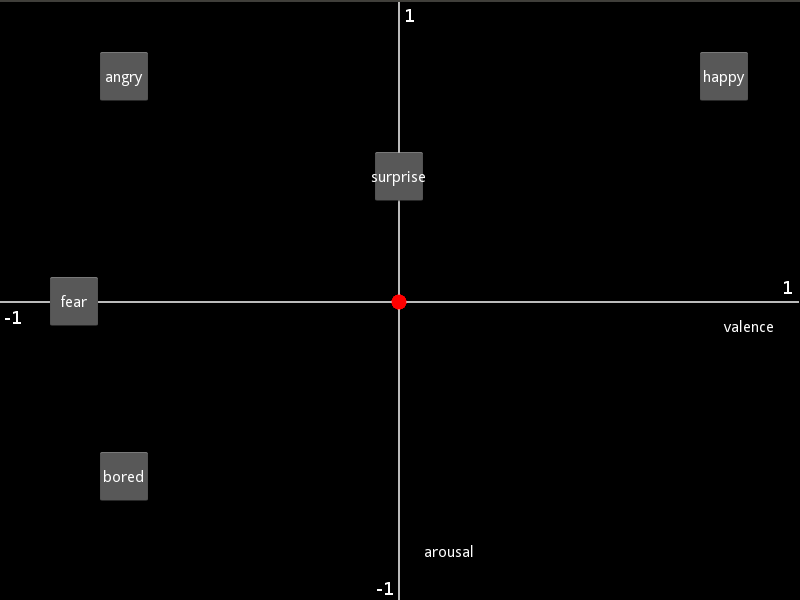
\includegraphics[width=.8\textwidth]{figures/vectMap.png}};

		\draw[->, color=green, thick] (0,0) -- (2,1.5);
		\draw[->, color=yellow, thick] (0,0) -- (0,1.2);
		\draw[->, color=blue, thick] (0,0) -- (-1.5,-1);
		\draw[->, color=red, thick] (0,0) -- (-1,0.75);
		\draw[red,fill=red] (0,0) circle (.8ex);
		
		\draw[white, thick,dashed] (0,3.5) ellipse (1cm and 0.5cm);
		\node[white, text width=2cm] at (0.6,3.45) {\tiny
		Saliency
		};
		
		\draw[white, thick,dashed] (-2,-2.5) ellipse (1.5cm and 1cm);
		\node[white, text width=2.5cm] at (-1.7,-2.5) {\tiny
		Time activity
		
		Number repetitions
		Ignoring
		};
		
		\draw[white, thick,dashed] (3.5,2) ellipse (1.5cm and 1cm);
		\node[white, text width=1.5cm] at (3.7,2) {\tiny
		Smiling
		
		Eye contact		
		Proximity
		};
		
		\draw[white, thick,dashed] (-2.4,2.5) ellipse (1cm and 0.5cm);
		\node[white, text width=2cm] at (-2,2.45) {\tiny		
		High QoM	
		};
	\end{tikzpicture}
    \caption{Valence and arousal map with all features compressed between -1 and 1}
    \label{fig:vectMap}
\end{figure}

\subsection{Direction and weighting}
The direction of the marker that defines the current behaviour (see red dot in figure \ref{fig:vectMap}) depends on the fusion of all different features with their respective weights. The formula that computes the resulting valence and arousal values provided to the action node is shown in \ref{eq:weight}.

\begin{equation}
 \vec{P_{t}}(val,aro) = \sum_{i=1}^N\vec{F}_{i}(val,aro) \cdot w_i
\end{equation}\label{eq:weight}

where $\vec{P_{t}}(val,aro)$ is the vector that defines the behaviour at time \textit{t} encoded by valence and arousal values. It is based on the combination of all vector features $ \vec{F}_{i} $ multiplied by their respective weights \textit{w}.

\section{Action node}
Finally, this node is the interface with the robot actuators. This node has been designed to encode all resources shown in the list located in section \ref{listResources} into the map shown in figure \ref{fig:vectMap}.

In the case of the physical joints, they are distributed uniformly along the map taking into account the limitations of the joint angles. For instance, the behaviour that corresponds to the point \textit{(0.8,0.8)} in the valence/arousal map in figure \ref{fig:vectMap} would not only move the arms, showing a positive expression, but also the head in a upper position among others.

In this way, the result received from the \textit{emotion manager} node with range $ [-1,1] $ is used to access the correspondent position stored in a matrix (for LEDs, pitch and volume) as well as used to modify the available joints for a certain duration of time. For instance, the shoulder roll, both right and left, are constrained between $ -76\degree $ and $ 18\degree $ were the values are defined by the \textit{valence} multiplied by a certain scale factor. The different actuators depend directly on the valence-arousal values as follows: 

\begin{itemize}
\item Head pitch: The head position of the robot is influenced exclusively by the arousal value. The higher the value, the higher the head position.

\begin{figure}[h!]
        \centering
        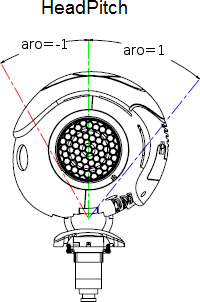
\includegraphics[width=0.2\textwidth]{figures/head.png}
        \caption{Head pitch boundaries for valence and arousal \cite{aldebaran}.}
        \label{fig:head}
\end{figure}

\item Shoulders pitch and roll: Shoulders have a pitch of +2 to -2 radians. Used in absolute mode, the central pitch value is 1.4 radians. It is exclusively modified by the valence value.

\begin{figure}[h!]
        \centering
        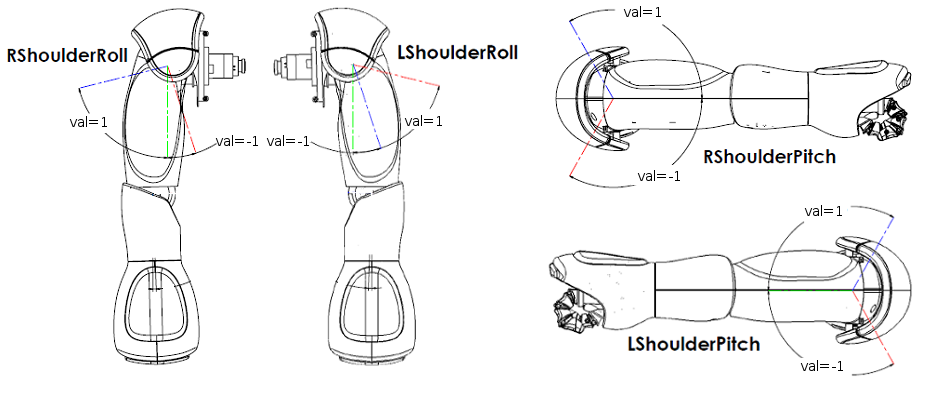
\includegraphics[width=0.8\textwidth]{figures/parts.png}
        \caption{Shoulder pitch and roll boundaries \cite{aldebaran} for valence and arousal.}
        \label{fig:parts}
\end{figure}

\item Pitch and volume: A matrix of 11x11 tuples was designed to keep the information of both pitch and volume. In this case, this feature is only modified by a the arousal value since the fundamental frequency of voice, speech rate and speech volume of the voice all seem to be related to the arousal of the emotion felt \cite{banse1996acoustic}. The values are integers of range $ [-1,1] $. 
\item LEDs: The same kind of matrix (in hexadecimal) was used to modify the eye colors. An example can be found in matrix \ref{eq:matrices}. In this case too, the color is defined by an arousal value since red colours are associated with high arousal emotions whereas blue ones with low arousal \cite{elliot2014color}.

\vspace{0.5cm}

\end{itemize}
\begin{equation}\label{eq:matrices}
M =  \begin{bmatrix} 
		\textcolor{red}{0xF82C35} & \textcolor{red}{0xF82C35} & \textcolor{RedOrange}{0xD55528} & \textcolor{RedOrange}{0xD55528} & ... & \textcolor{green}{0x56C427}  \\
		\textcolor{red}{0xF82C35} & \textcolor{red}{0xF82C35} & \textcolor{BurntOrange}{0xD5542A} & \textcolor{BurntOrange}{0xD5542A} & ... & \textcolor{ForestGreen}{0x56C427}  \\
		\textcolor{BrickRed}{0xF62D35} & \textcolor{BrickRed}{0xF62D35} & \textcolor{BrickRed}{0xF62D35} & \textcolor{Bittersweet}{0xE96A37} & ... & \textcolor{JungleGreen}{0x56C427}  \\
			:	 &	:		&		:  &		: & :   & 		: 	  \\
		\textcolor{Fuchsia}{0x692850} & \textcolor{Fuchsia}{0x692850} & \textcolor{Fuchsia}{0x692850} & \textcolor{Fuchsia}{0x692850} & ... & \textcolor{MidnightBlue}{0x0085BE}		
	 \end{bmatrix}_{11x11}
\end{equation}

\vspace{0.5cm}

It is important to notice that not all feature actions are executed continuously during the activities. This is the case only of the volume and pitch and the color changing. The rest of the movements are performed in specific times to avoid collisions with the current activity, for instance, the arm movement in the writing process  Most of them are applied during the \textit{waiting for feedback} state shown in figure \ref{fig:stateMachine}. Furthermore, a face tracking is performed continuously in order to provide eye contact with the user, using \textit{ALFaceDetection} from NaoQi, which is based on a commercial face detection solution.

\section{Results}
The result of the adaptive behaviour model \footnote{https://github.com/chili-epfl/emotional-manager} is shown in figure \ref{fig:behaviours}. 

\begin{figure}[h!]
        \centering        
        \begin{subfigure}[b]{0.18\textwidth}
                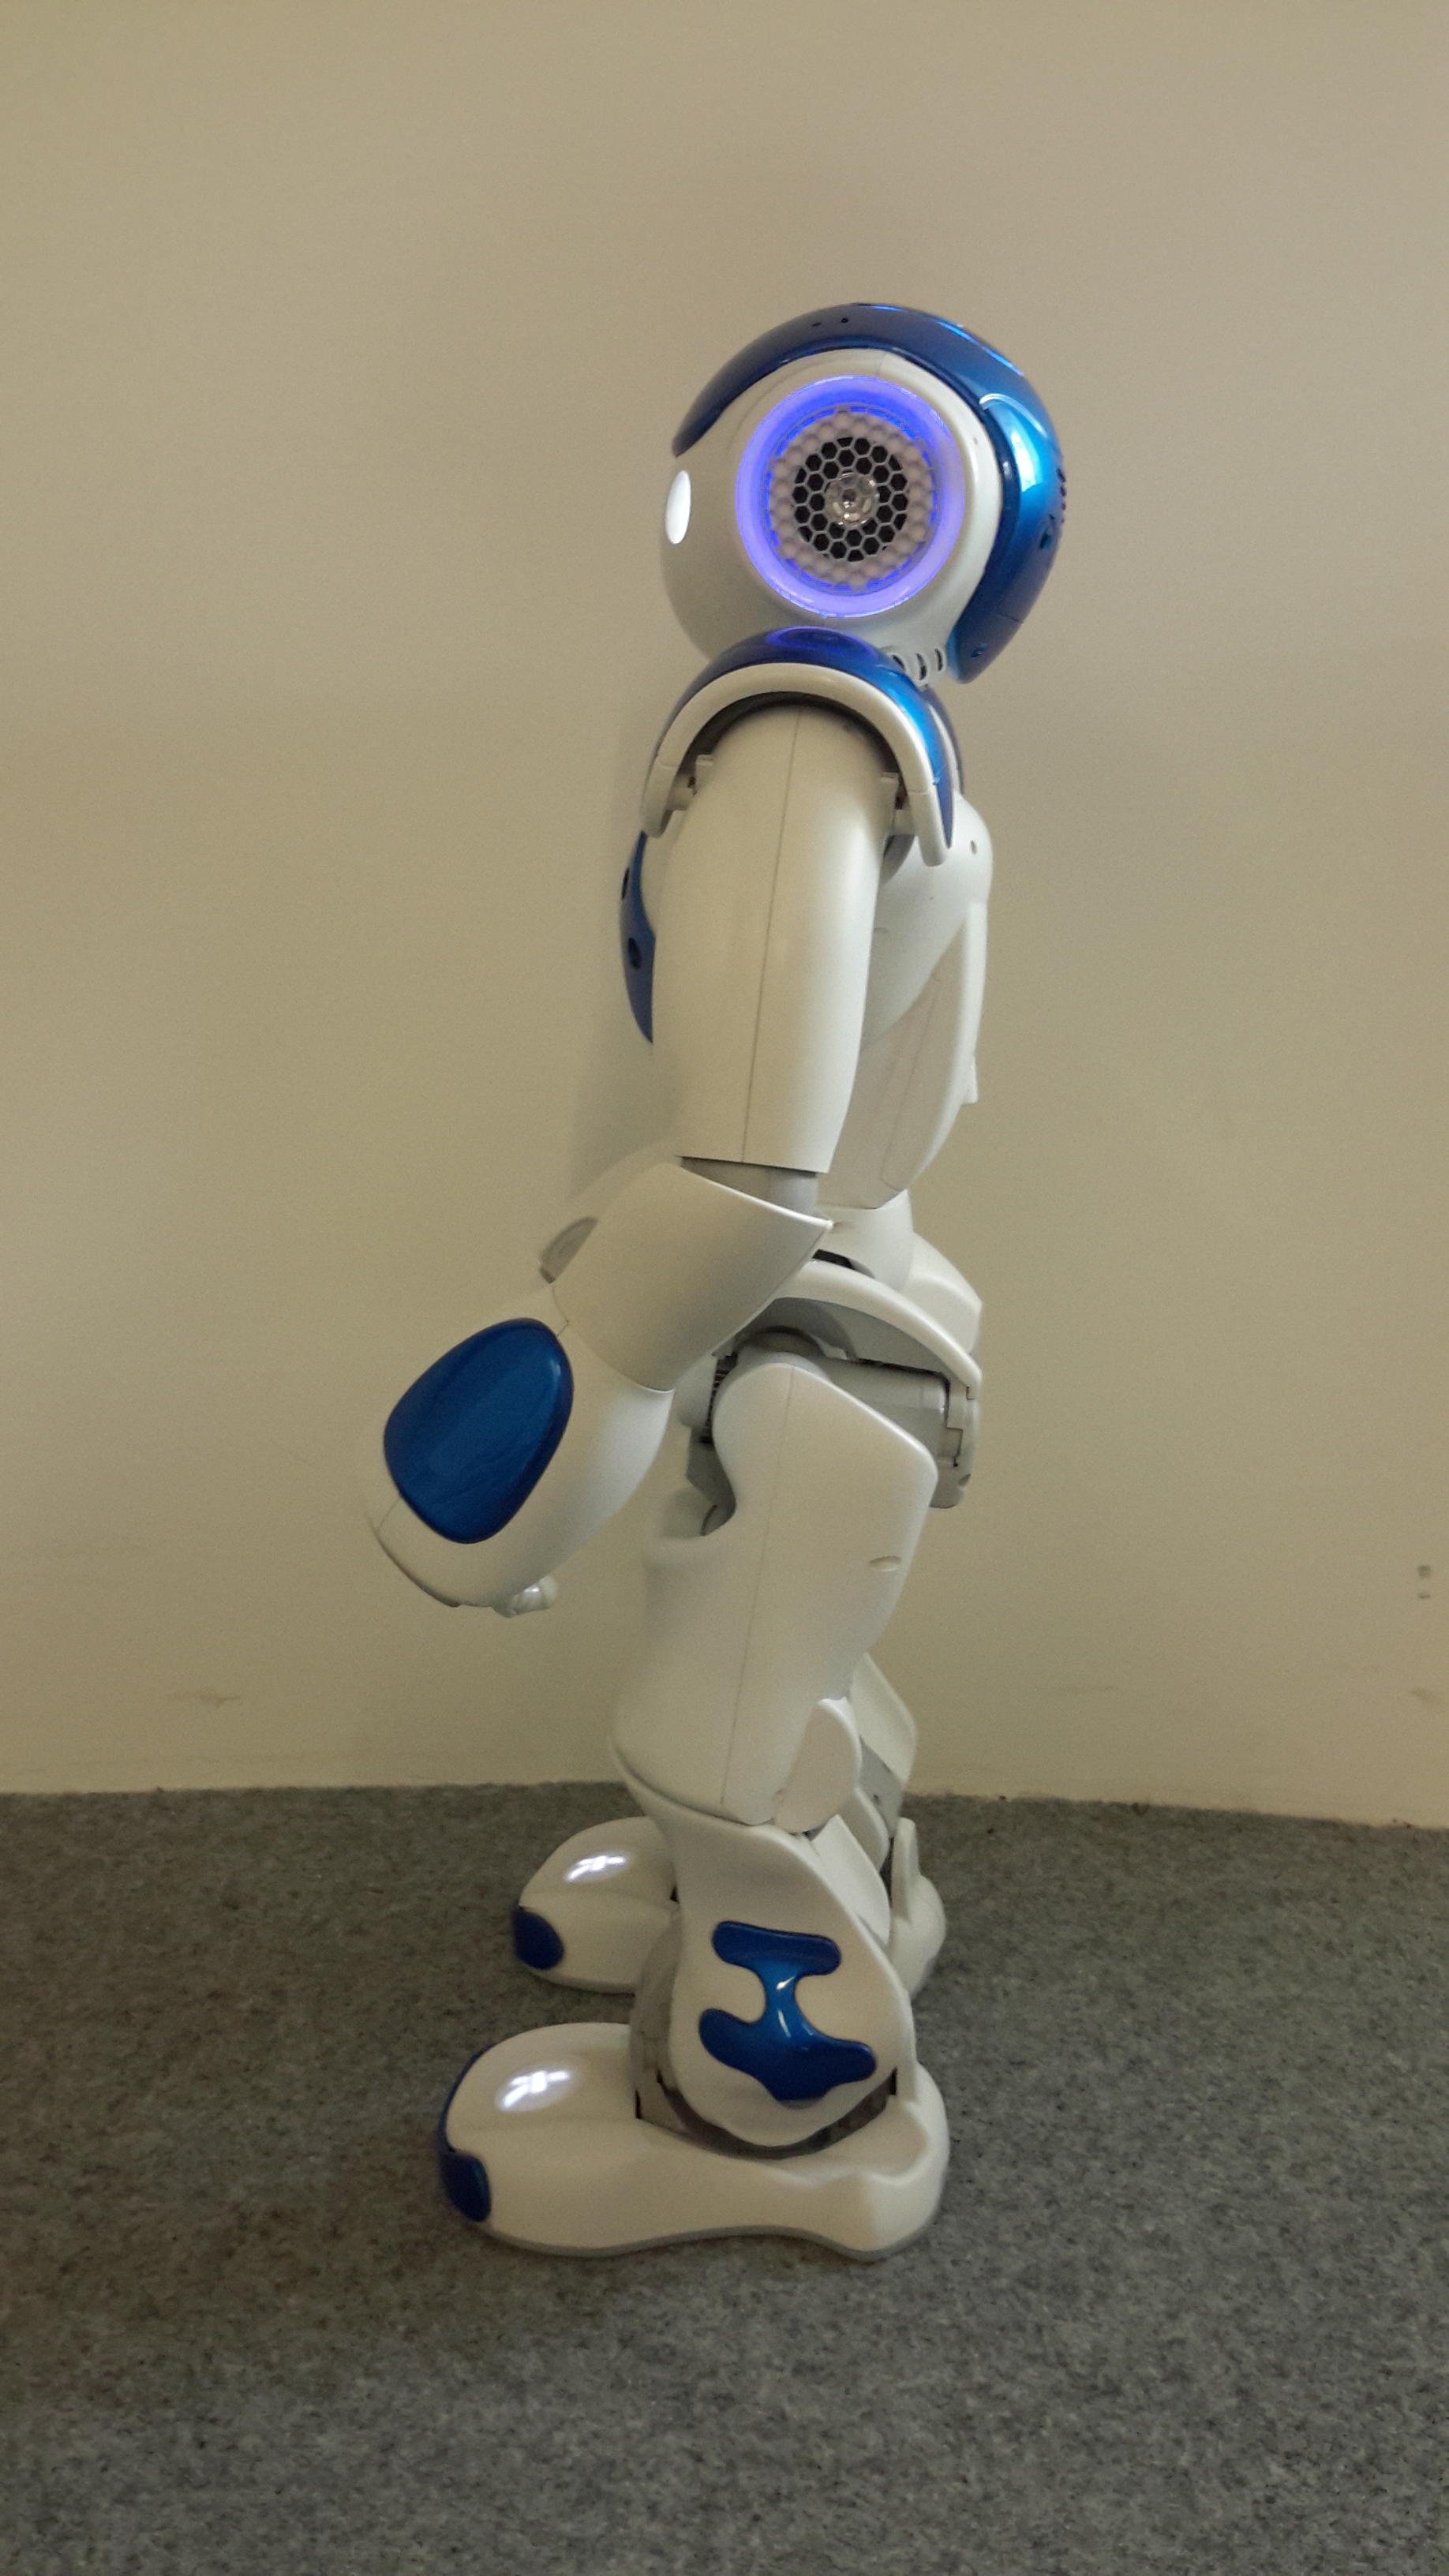
\includegraphics[width=\textwidth]{figures/neutral.jpg}
                \caption{Neutral}
                \label{fig:neutral}
        \end{subfigure}
        ~ %add desired spacing between images, e. g. ~, \quad, \qquad, \hfill etc.
          %(or a blank line to force the subfigure onto a new line)
        \begin{subfigure}[b]{0.18\textwidth}
                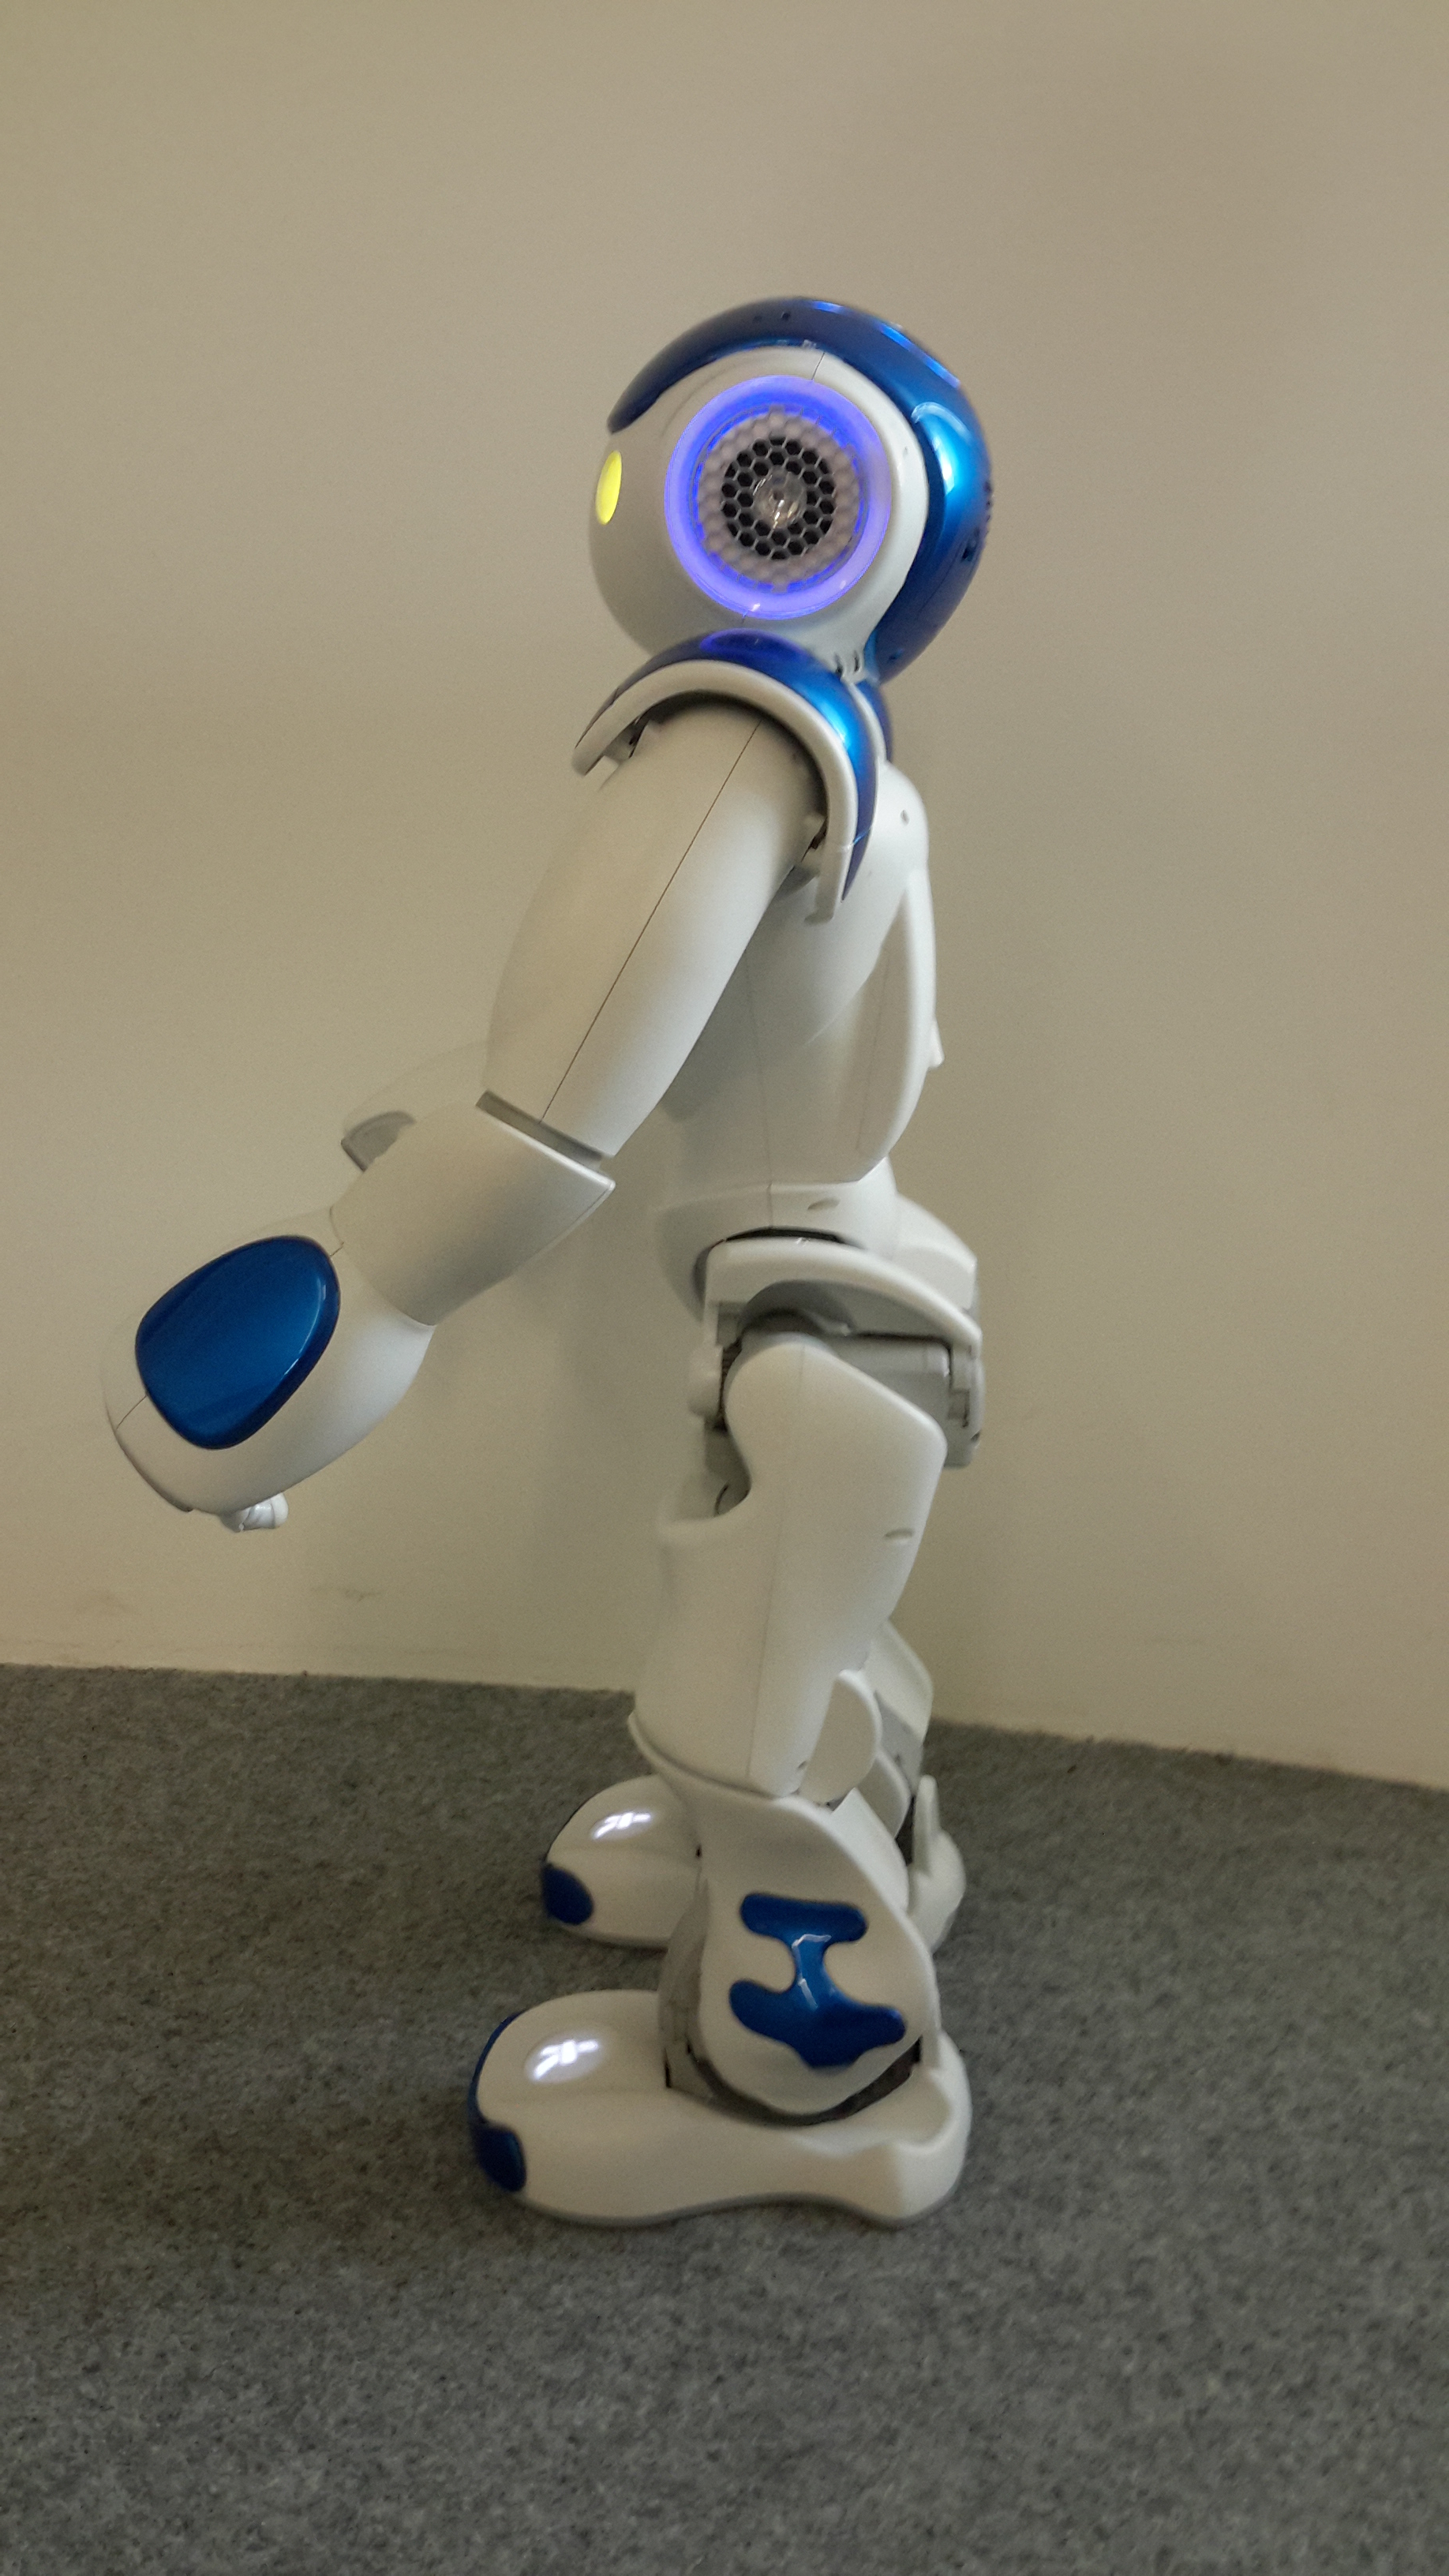
\includegraphics[width=\textwidth]{figures/happy.jpg}
                \caption{Happy}
                \label{fig:happy}
        \end{subfigure}%
        ~ %add desired spacing between images, e. g. ~, \quad, \qquad, \hfill etc.
          %(or a blank line to force the subfigure onto a new line)
        \begin{subfigure}[b]{0.18\textwidth}
                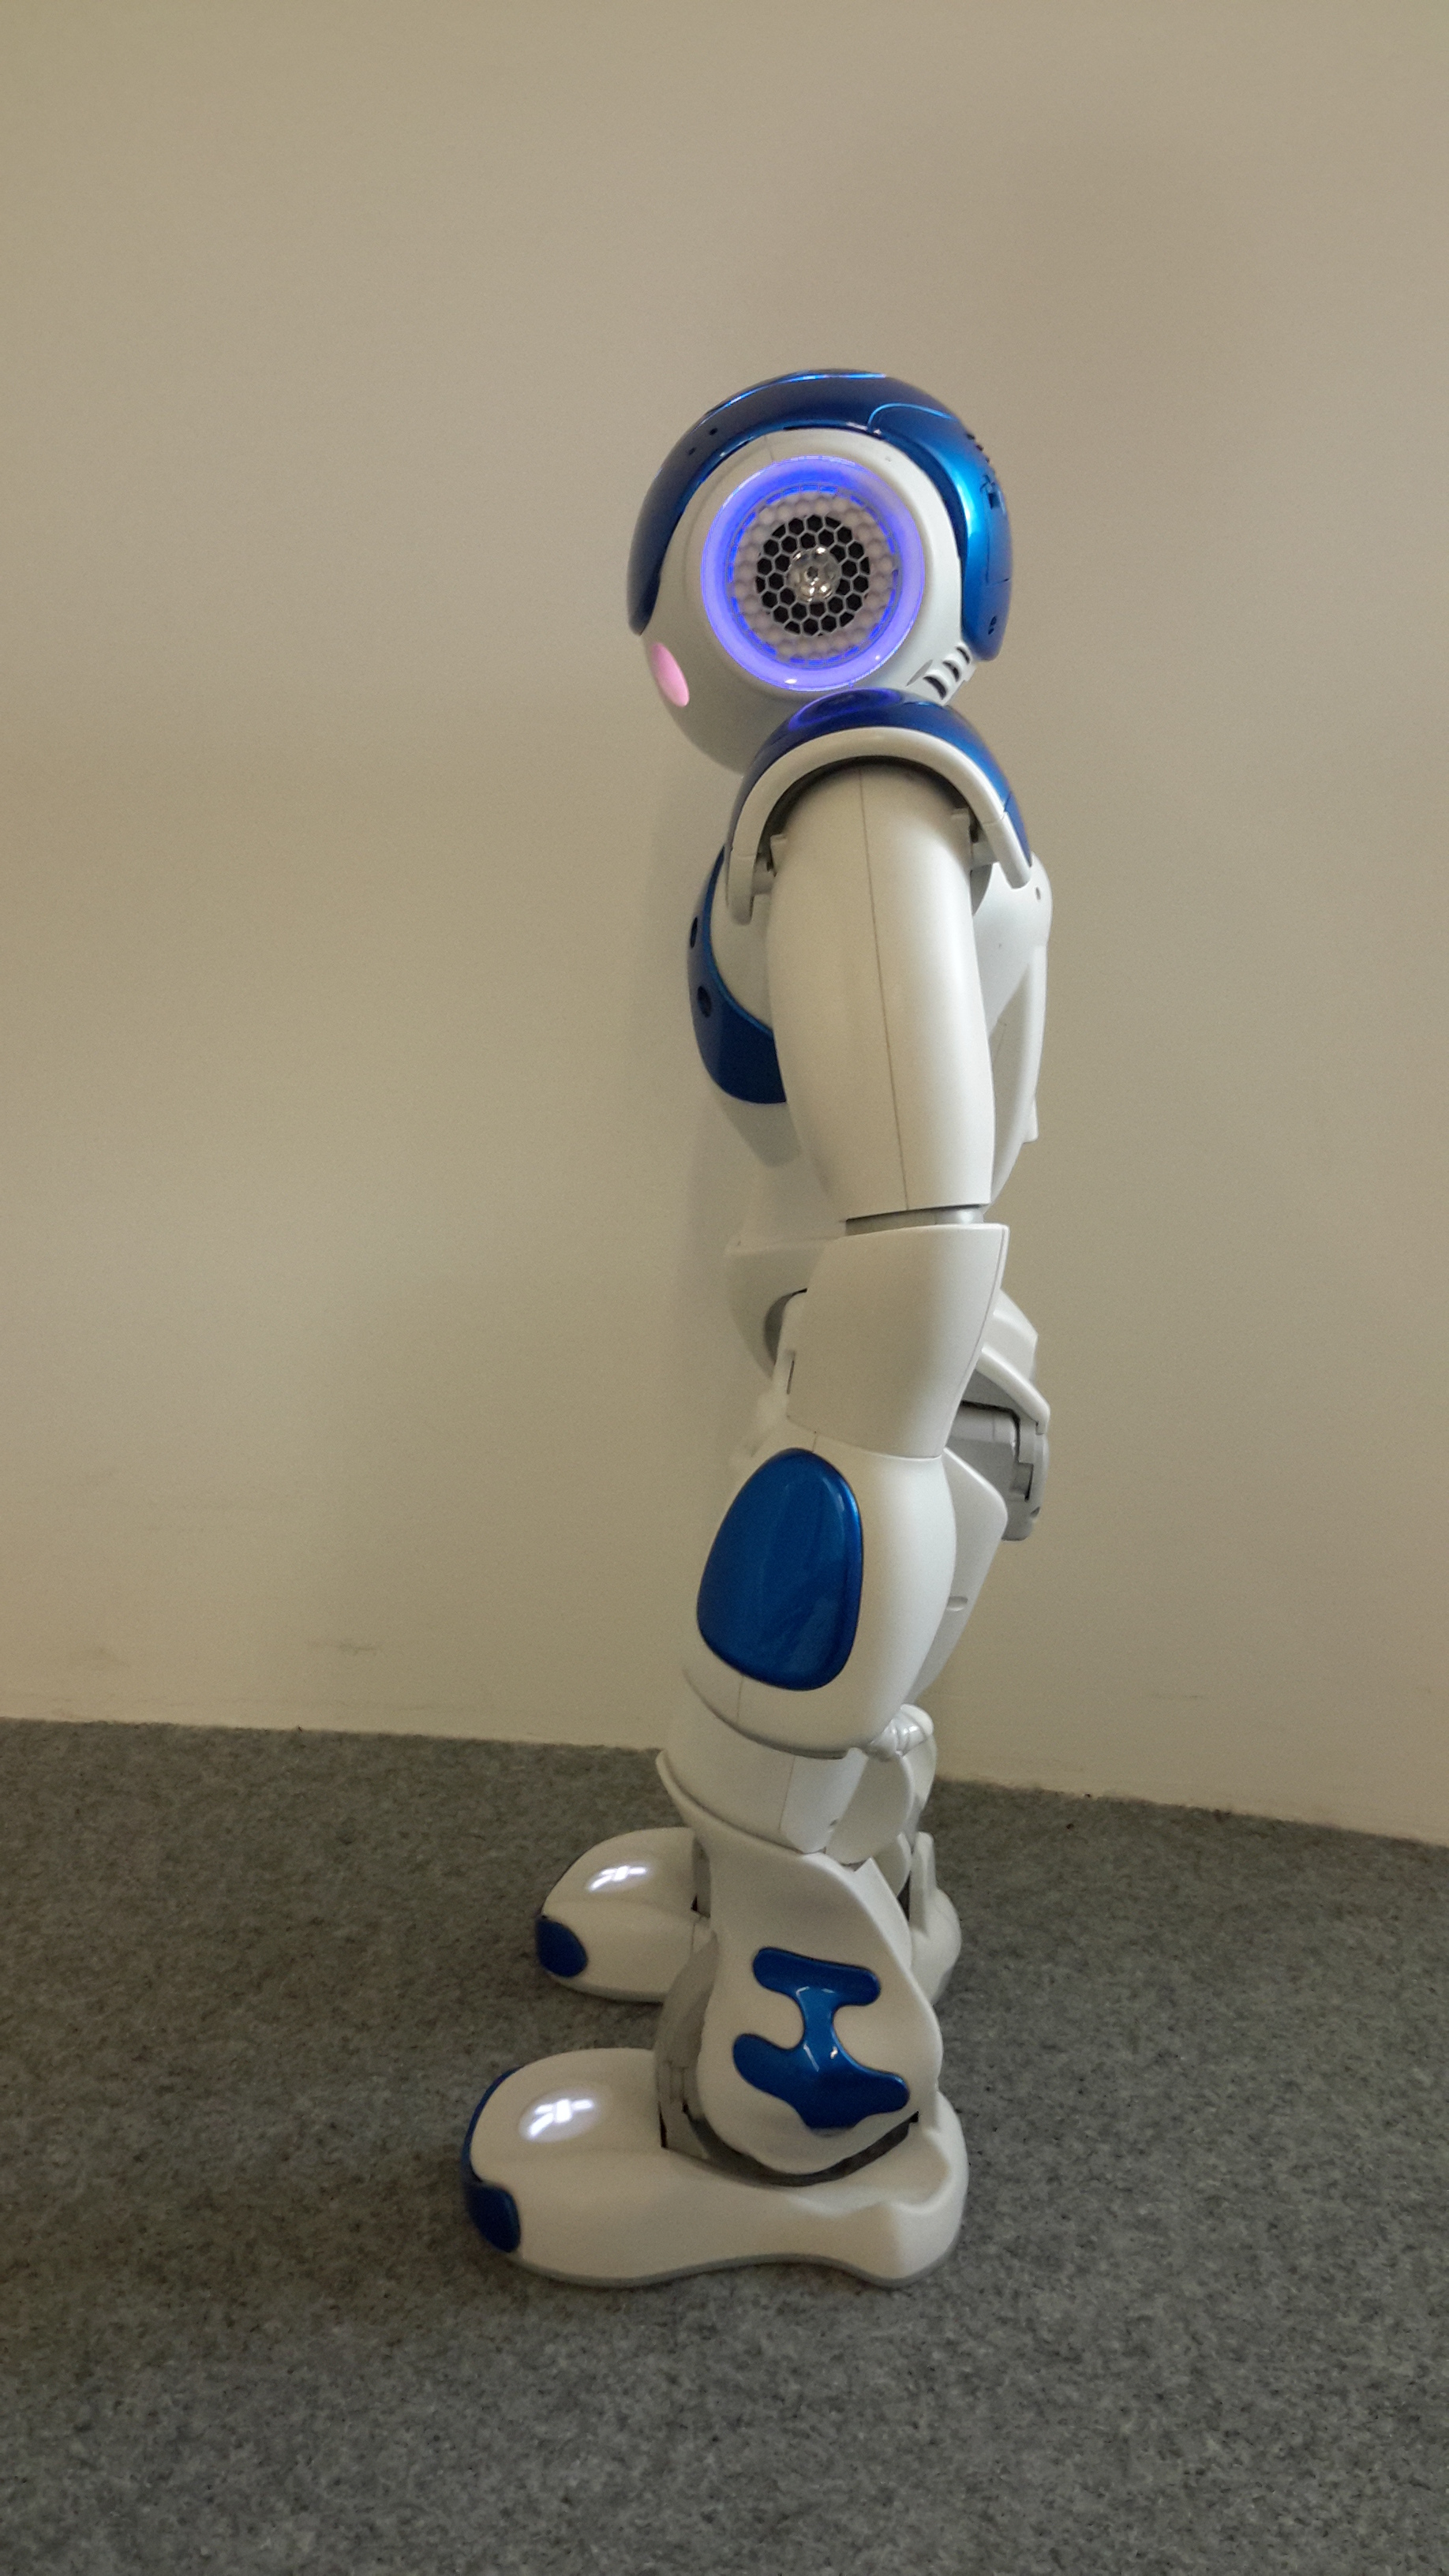
\includegraphics[width=\textwidth]{figures/sad.jpg}
                \caption{Sad}
                \label{fig:sad}
        \end{subfigure}
        ~ %add desired spacing between images, e. g. ~, \quad, \qquad, \hfill etc.
          %(or a blank line to force the subfigure onto a new line)
        \begin{subfigure}[b]{0.18\textwidth}
                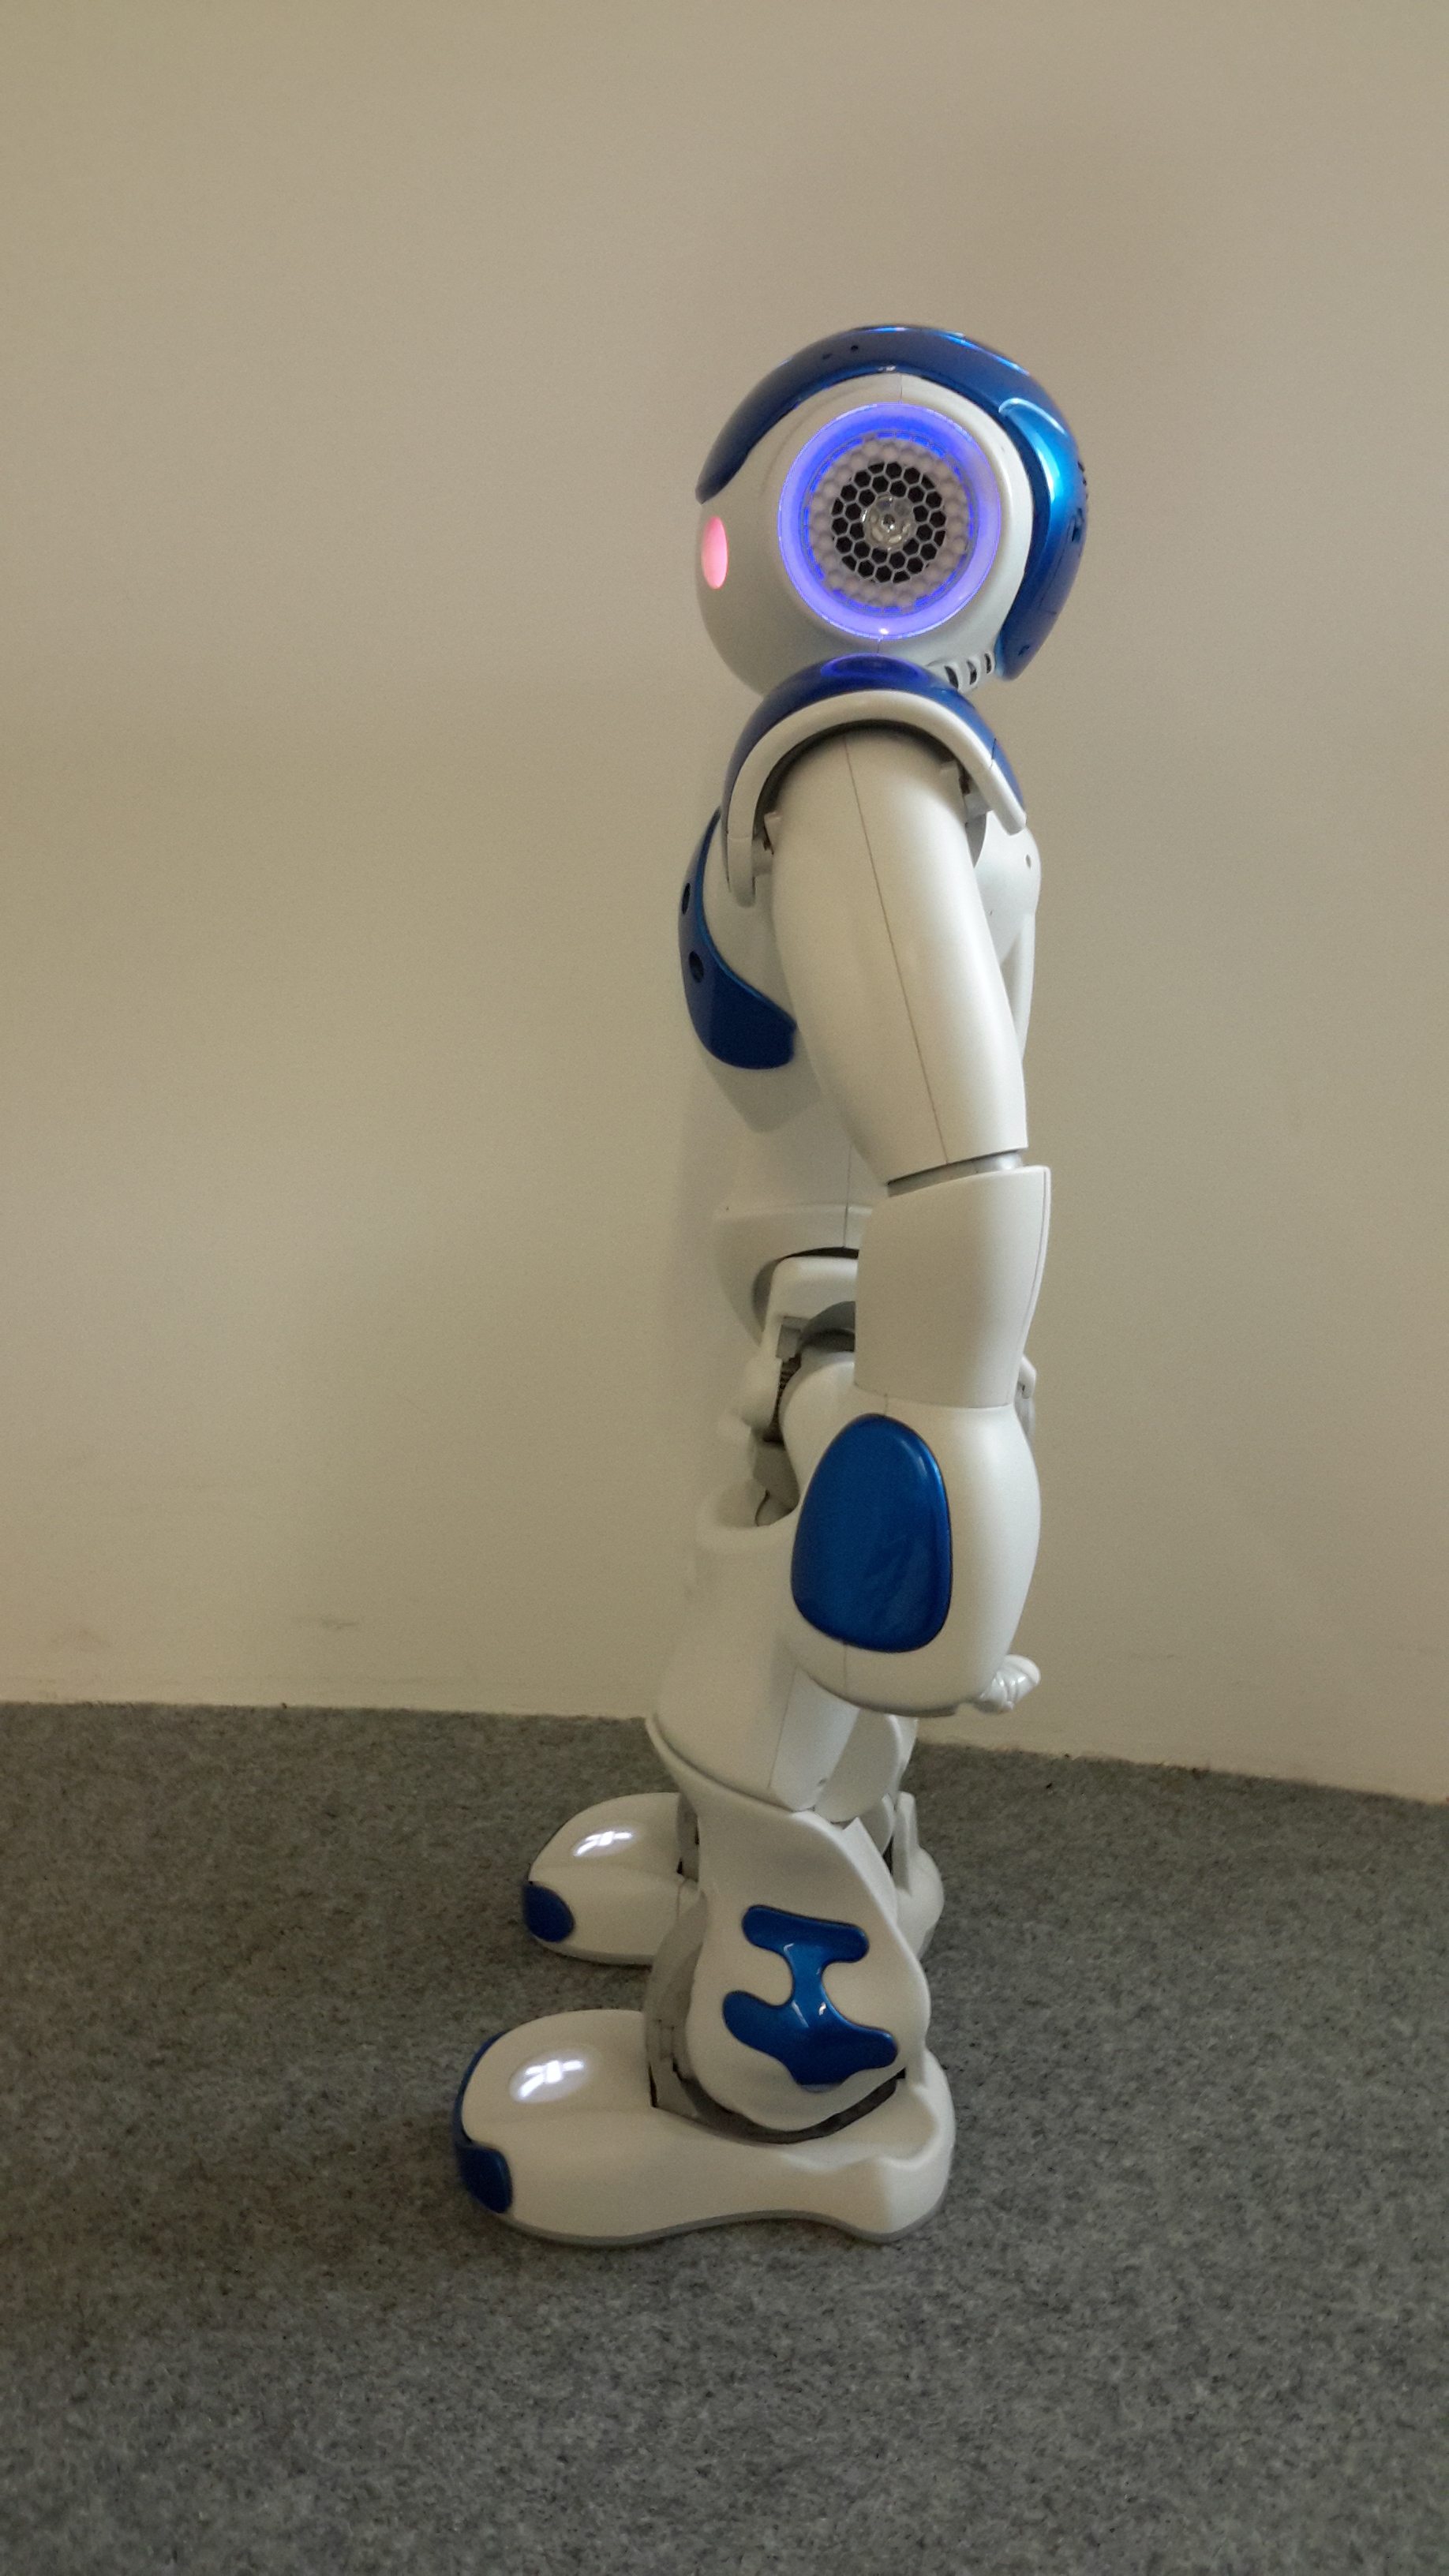
\includegraphics[width=\textwidth]{figures/bored.jpg}
                \caption{Bored}
                \label{fig:bored}
        \end{subfigure}
        ~ %add desired spacing between images, e. g. ~, \quad, \qquad, \hfill etc.
          %(or a blank line to force the subfigure onto a new line)
        \begin{subfigure}[b]{0.18\textwidth}
                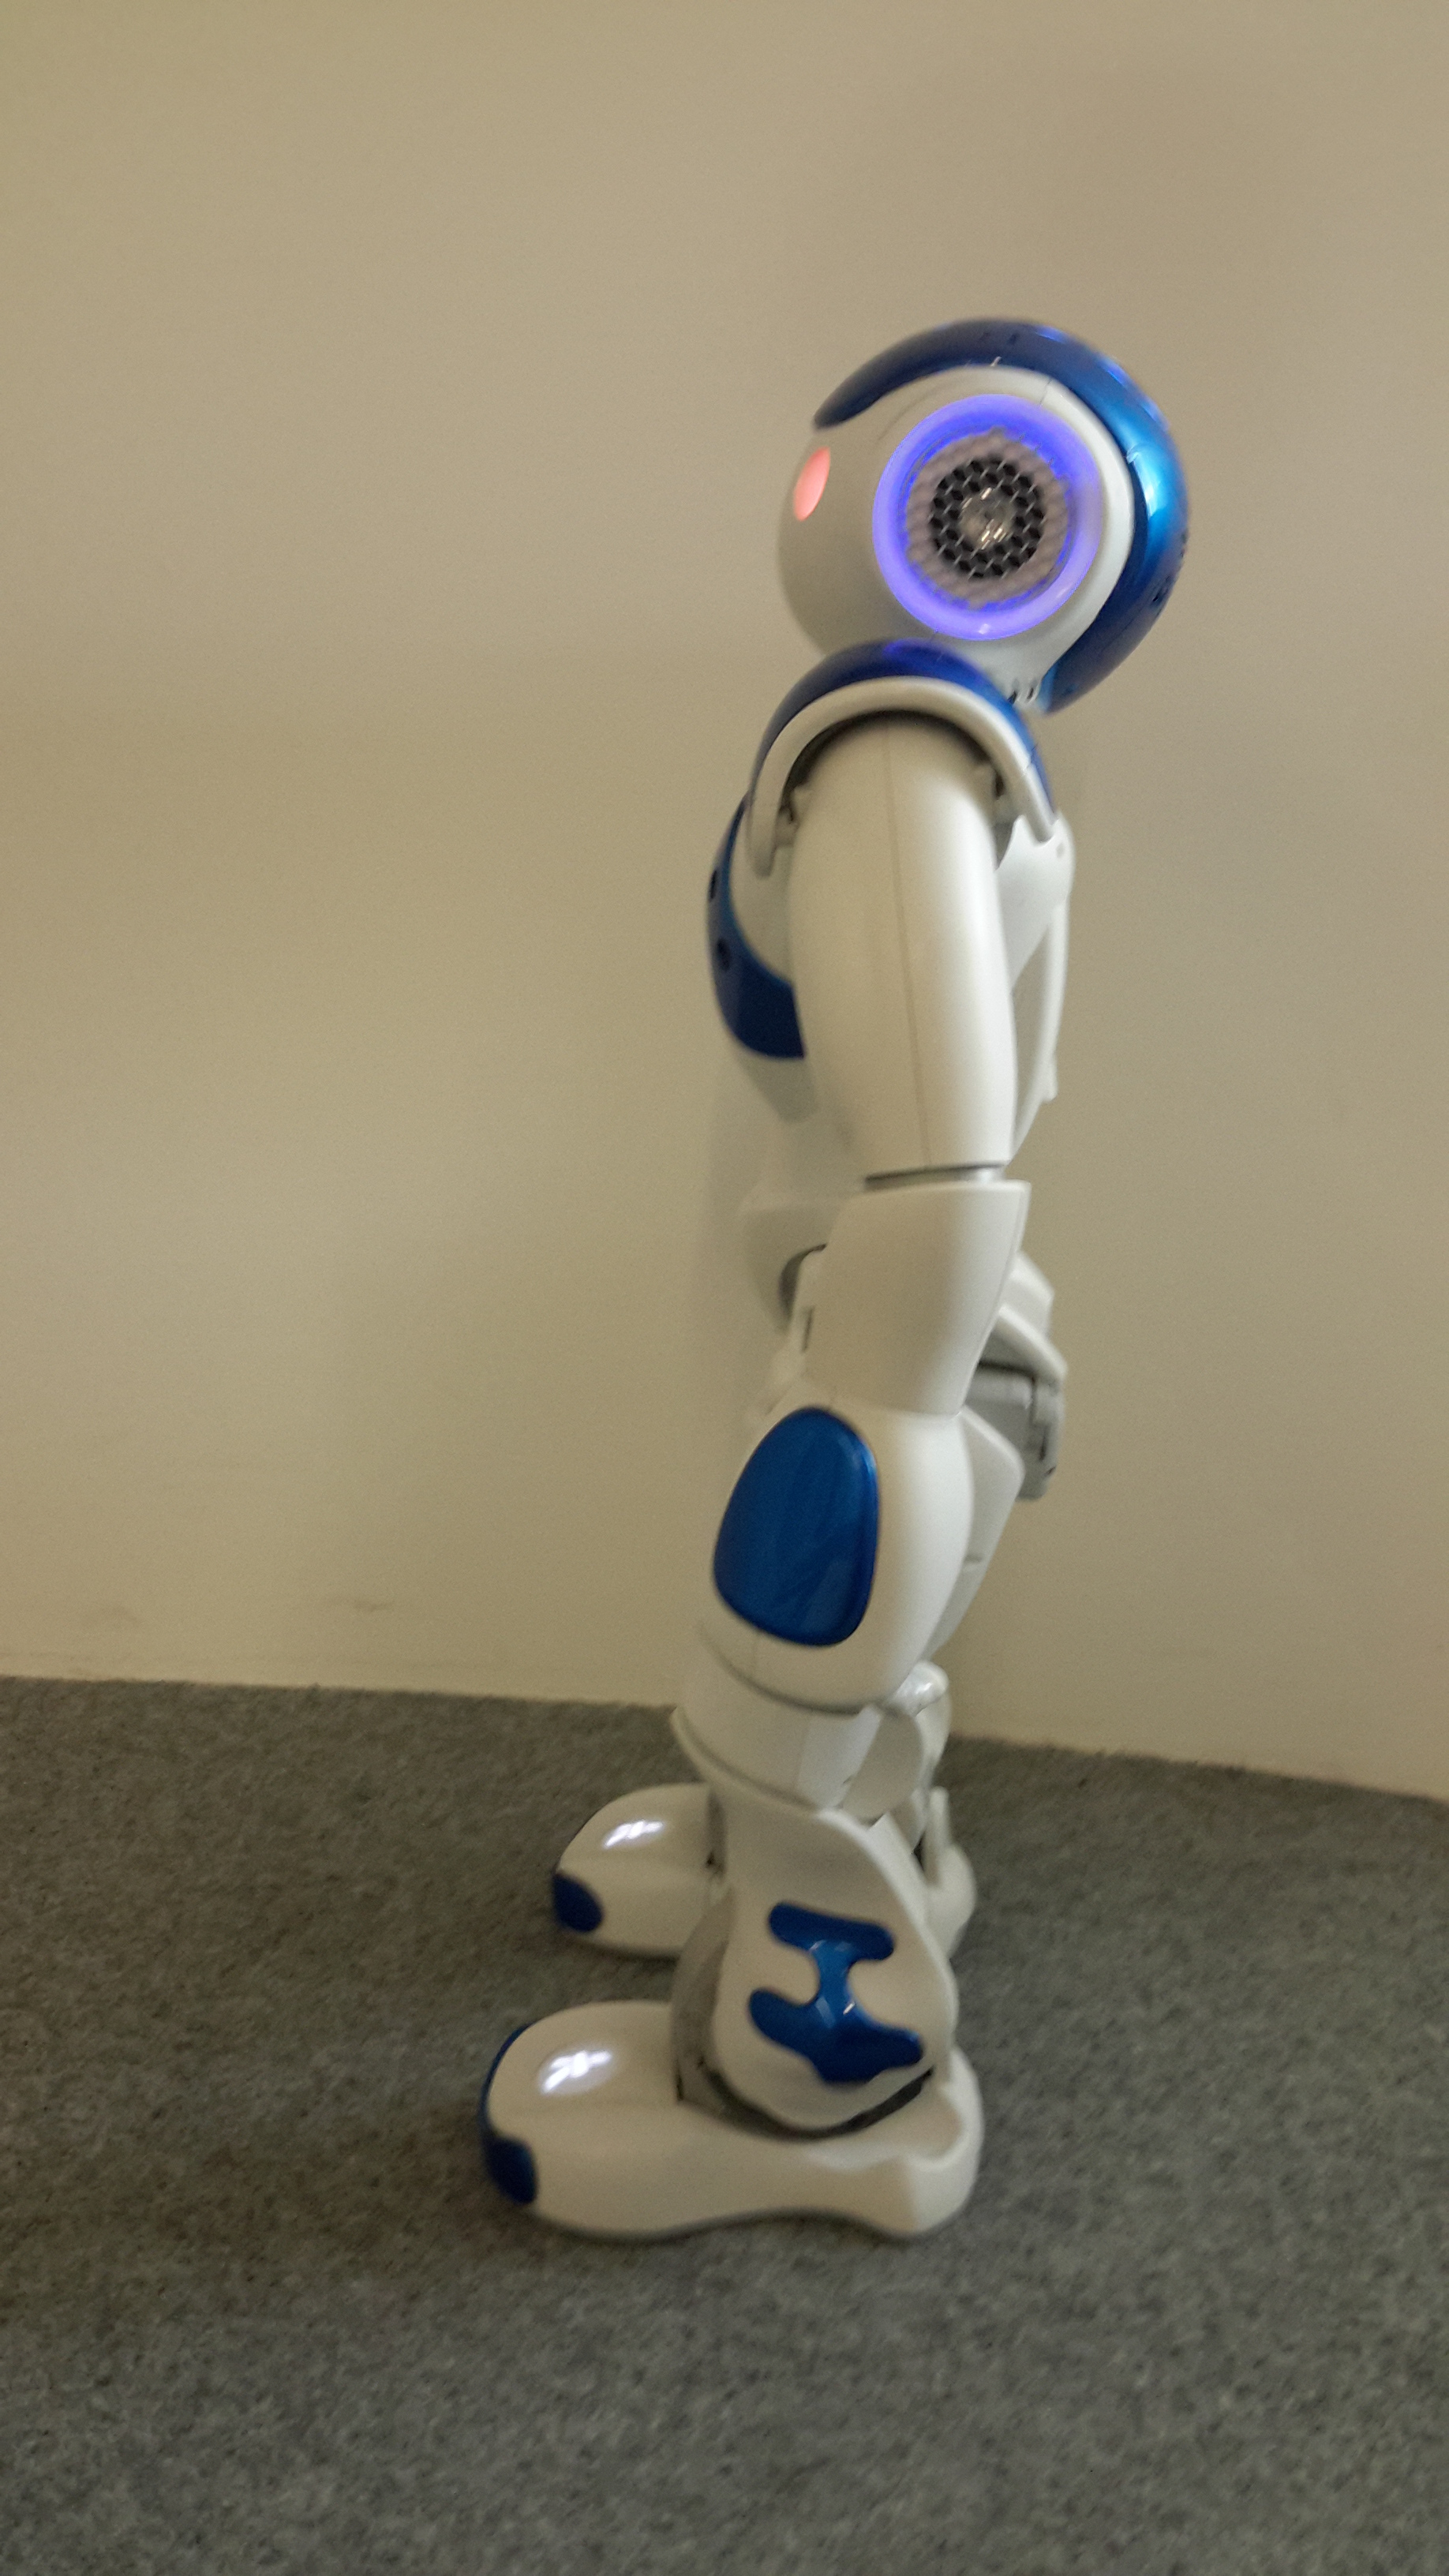
\includegraphics[width=\textwidth]{figures/angry.jpg}
                \caption{Angry}
                \label{fig:angry}
        \end{subfigure}
		\caption{Examples of behaviours generated by the valence-arousal model}\label{fig:behaviours}
\end{figure}
